\documentclass[12pt,a4paper]{scrartcl}

\usepackage{graphicx}
\usepackage{amsmath}
\usepackage{amsfonts}
\usepackage{amssymb}
\usepackage{bm}
\usepackage{ulem}
\let\mathbf\bm


\usepackage[T1]{fontenc}
\usepackage[utf8]{inputenc}
\usepackage[magyar]{babel}
\usepackage{lmodern}

\usepackage{placeins}
\usepackage{subcaption}
\usepackage{epstopdf}
\usepackage{xcolor}
\usepackage[hidelinks,unicode]{hyperref}
\hypersetup{
    colorlinks,
    linkcolor={red!50!black},
    citecolor={blue!50!black},
    urlcolor={blue!80!black}
}

\usepackage{cleveref}




\begin{document}
\title{Hőtan és folytonos közegek mechanikája\\(emelt szint)}
\author{hotanef19va, gyakorlat,\\Anyagfizikai Tanszék, Tüzes Dániel}
\maketitle
\tableofcontents

\iffalse %csak akkor használd, ha nincs további if belül
\section{Sűrűséges feladatok}
\subsection{Rúd sűrűsége}
Egy rúd sűrűsége a hely függvényében legyen $\rho \left( x \right) = c/{x^2}$.
\begin{enumerate}
\item Milyen típusú sűrűségre gondolt az, aki egy ilyen példát kitűz?
\item Mi lehet $c$ dimenziója?
\item Mi a rúd tömege a
\begin{itemize}
\item $\left[ 1{\text{ m, }}2{\text{ m}} \right]$,
\item $\left( 1{\text{ m, }}2{\text{ m}} \right)$,
\item ${\left( {0{\text{ m, }}1{\text{ m}}} \right)}$ és
\item ${\left[ {0{\text{ m, }}1{\text{ m}}} \right]}$ között?
\end{itemize}
\item Létezhet-e ilyen sűrűségű lemez?
\end{enumerate}
\subsection{Levegő sűrűsége}
A levegő sűrűsége legyen a $h$ magasság függvényében $\rho \left( h \right) = {\rho _0} \cdot {e^{ - c \cdot h}}$.
\begin{enumerate}
\item Mi $c$ és $\rho_0$ dimenziója?
\item Hanyad részére csökken adott térfogatú levegő tömege $L$-lel magasabban, ha a térfogat befoglaló gömbjének átmérője $ \ll \frac{1}{c}$?
\end{enumerate}

\subsection{Áramerősség}
Legyen az áramsűrűség-mező ${\mathbf{j}}\left( {\mathbf{r}} \right) = c \cdot {\mathbf{r}}/{r^3}$.
\begin{enumerate}
\item Mi $c$ dimenziója?
\item Mennyi töltés halad át az $1\text{ m}$ sugarú gömbön? És a $2\text{ m}$ sugarún?
\item Mennyi töltés halad át azon a négyzeten, aminek a négy sarkának a koordinátái: ${{\mathbf{r}}_A} = \left( {1,0,0} \right)$, ${{\mathbf{r}}_B} = \left( {1,1,0} \right)$, ${{\mathbf{r}}_C} = \left( {1,1,1} \right)$ és ${{\mathbf{r}}_D} = \left( {1,0,1} \right)$?
\end{enumerate}
\fi

\section{Merev testek}
\subsection{Négyféle tenzor}
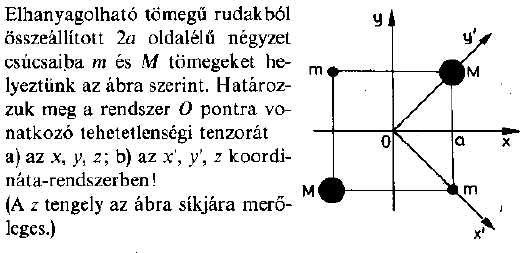
\includegraphics[scale=0.8]{lusta/merev_test1pelda.png}

A c) és d) alfeladatokhoz számold ki az egyik $M$ tömegű testbe helyezett origóra a tehetetlenségi nyomaték tenzort az a) és a b) esetekben párhuzamos tengelyekre!

\subsection{Integrális rúd}
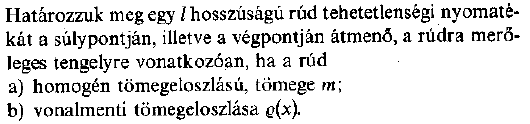
\includegraphics[scale=0.8]{lusta/merev_test2pelda.png} 

A rúd elég vékony, a hossztengelye mentén egy szakasszal modellezhető ebben a feladatban.

\section{Egyszerű transzformációk I}
\subsection{Eltolás otthon}
Legyen a testünk $A$ és $B$ pontjainak koordinátáira ${{\mathbf{r}}_A} = \left( { - 10, - 1} \right)$ és ${{\mathbf{r}}_B} = \left( { 3, 3} \right)$, valamint $\Delta {\mathbf{r}} = {{\mathbf{r}}_B} - {{\mathbf{r}}_A}$! Legyen az elmozdulásmező ${\mathbf{u}}\left( {\mathbf{r}} \right) = \left( { - 2, - 2} \right)$. Mennyi a disztorzió és annak szimmetrikus illetve antiszimmetrikus része, a deformációs gradiens, a deformáció és a relatív térfogatváltozás? Számold ki $\Delta {\mathbf{r}}'$ értékét is!
\subsection{Nyújtás otthon}
\begin{enumerate}
\item Legyen a testünk $A$ és $B$ pontjainak koordinátáira ${{\mathbf{r}}_A} = \left( { - 3, - 0.5} \right)$ és ${{\mathbf{r}}_B} = \left( { - 0.5, - 0.5} \right)$, valamint $\Delta {\mathbf{r}} = {{\mathbf{r}}_B} - {{\mathbf{r}}_A}$! Végezzünk el egy képlékeny deformációt, amelynek során
\[\begin{aligned}
  x' &  = 2 \cdot x \\ 
  y' &  = \lambda \cdot y \\ 
  z' &  = \lambda  \cdot z. \\ 
\end{aligned} \]

Mennyi a disztorzió és annak szimmetrikus illetve antiszimmetrikus része, a deformációs gradiens, a deformáció és a relatív térfogatváltozás? Add meg $\Delta {\mathbf{r}}'$ értékét is!

Mennyi legyen $\lambda$, hogy a relatív térfogatváltozás 0 legyen? Mennyi ekkor a disztorzió és annak szimmetrikus illetve antiszimmetrikus része, a deformációs gradiens, a deformáció? Add meg $\Delta {\mathbf{r}}'$ értékét is és készíts rajzot!

\item Legyen a testünk $A$ és $B$ pontjainak koordinátáira ${{\mathbf{r}}_A} = \left( { - 3, - 0.5} \right)$ és ${{\mathbf{r}}_B} = \left( { - 0.5, - 0.5} \right)$, valamint $\Delta {\mathbf{r}} = {{\mathbf{r}}_B} - {{\mathbf{r}}_A}$! Legyenek az új koordináták
\[\begin{aligned}
  x' &  = 2 \cdot x \\ 
  y' &  = 3 \cdot y \\ 
  z' &  = 1 \cdot z. \\ 
\end{aligned} \]

Írd fel az elmozdulásmezőt vektoros alakban! Mire változik a $\Delta {\mathbf{r}}$ vektor? Mennyi a disztorzió, a deformációs gradiens és a relatív térfogatváltozás?

Tegyük át az origót az $A$ pontba és írjuk le innen is a nyújtást! Legyenek a vektoraink a csillagosak, ${{\mathbf{r}}_A}^*$ és ${{\mathbf{r}}_B}^*$. Hogyan változnak transzformációra általánosan a vektorok? Azaz add meg az ${\mathbf{r}}{{^*}'}\left( {{{\mathbf{r}}^ * }} \right)$ függvényt! Mi az elmozdulástér, a disztorzió, a $\Delta {{\mathbf{r}}^ * }'$, a deformációs gradiens és a relatív térfogatváltozás? Készíts rajzot is!
\end{enumerate}

\iffalse
\subsection{Nem origó körüli}
Adottak az alábbi transzformációk egy vonatkoztatási rendszerben, illetve  az $A$ és $B$ pontok, amelyekhez mutató vektorok ${{\mathbf{r}}_A} = \left( {1,0} \right)$ és ${{\mathbf{r}}_A} = \left( {0, - 1} \right)$. Add meg az eredeti, illetve az új vonatkoztatási rendszerben az elmozdulásmezőt, a $\Delta {{\mathbf{r}}_{AB}}$ vektort, a disztroziót, a deformációs gradienst és a deformációt!
\begin{enumerate}
\item Eltolás: ${\mathbf{u}}\left( {\mathbf{r}} \right) = {{\mathbf{r}}_0}$
\item Nyújtás: ${\mathbf{r}}'\left( {\mathbf{r}} \right) = \left( {2 \cdot {{\mathbf{e}}_x} \circ {{\mathbf{e}}_x} + 1 \cdot {{\mathbf{e}}_y} \circ {{\mathbf{e}}_y} + {{\mathbf{e}}_z} \circ {{\mathbf{e}}_z}} \right){\mathbf{r}}$
\item Forgatás: ${\mathbf{r}}'\left( {\mathbf{r}} \right) = {\mathbf{Or}}\quad {\mathbf{O}} = {{\mathbf{O}}_{z,45^\circ }} = \left( {\begin{array}{*{20}{c}}
  {\cos \left( {45^\circ } \right)}&{ - \sin \left( {45^\circ } \right)}&0 \\ 
  { - \sin \left( {45^\circ } \right)}&{\cos \left( {45^\circ } \right)}&0 \\ 
  0&0&1 
\end{array}} \right)$
\end{enumerate}

\subsection{Forgatás}
Mutassuk meg, hogy kicsi forgatásokra valóban felírható \begin{equation} \label{eq:inf_forgat}
{{\mathbf{u}}^f}\left( {\mathbf{r}} \right) = \Delta {\mathbf{\varphi }} \times {\mathbf{r}},
\end{equation}
alak az elmozdulásmezőre! Mutassuk meg, hogy véges nagyságú forgatásra is $0$ a deformáció!


\subsection{Konkrét számok}
Írjuk fel az alábbi esetekre at elmozdulásmezőt, a disztorziót, a deformációs gradienst és a deformációt! Hogyan néznek ki ezek (első rendű közelítésben), ha az adott fajtájú egyszerű transzformációk kicsik?

\begin{figure}[htb] 
\centering
\begin{subfigure}[b]{0.45\textwidth}
\centering
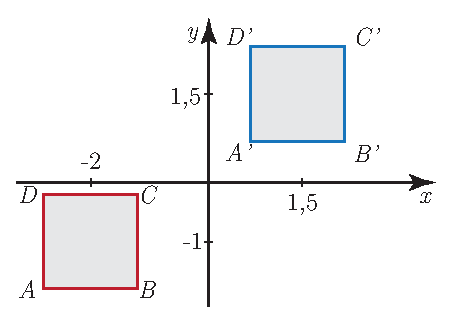
\includegraphics[scale=1]{figs/eltolas_feladat.eps}
\caption{Eltolás.}
\label{fig:eltolas_feladat}
\end{subfigure} \hfill
\begin{subfigure}[b]{0.45\textwidth}
\centering
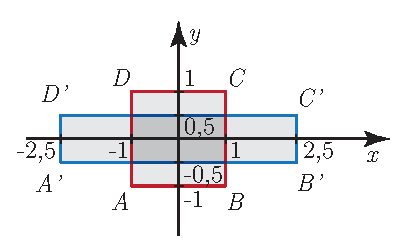
\includegraphics[scale=1]{figs/nyujtas_feladat.eps}
\caption{Nyújtás.}
\label{fig:nyujtas_feladat}
\end{subfigure}
\begin{subfigure}[b]{0.45\textwidth}
\centering
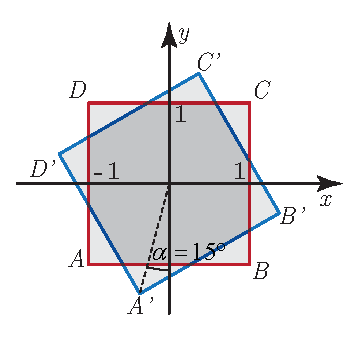
\includegraphics[scale=1]{figs/forgatas_feladat.eps}
\caption{Forgatás.}
\label{fig:forgatas_feladat}
\end{subfigure}
\label{fig:konret_szamos_feladat}
\caption{Konkrét számos feladat.}
\end{figure}
\FloatBarrier

\section{Egyszerű transzformációk II}
\subsection{Egyenes képe egyenes}
Mutassuk meg, hogy eltolás, nyújtás és forgatás során szakasz képe szakasz! Ehhez felhasználhatjuk, hogy az $A$ és $B$ pontok közötti $AB$ szakaszt a két pontba mutató ${{\mathbf{r}}_A}$ és ${{\mathbf{r}}_B}$ vektorokkal úgy írhatjuk fel, hogy 
\[AB = \left\{ {\left. {{\lambda _A}{{\mathbf{r}}_A} + {\lambda _B}{{\mathbf{r}}_B}} \right|{\lambda _A} + {\lambda _B} = 1} \right\}.\]

\subsection{Nyírós-számolós}
\begin{enumerate}
\item \Aref{fig:nyiras_feladat}.\ ábrán melyik fajta nyírás van ábrázolva? Mi az elmozdulásmező, a deformációs gradiens, a disztorzió és a deformáció?
\item Általános és tiszta (véges) nyírás eseteiben leolvasható-e (radiános) szögmérő segítségével a disztorzió komponensei? És infinitezimális transzformáció esetén?
\item Infinitezimális tiszta nyírásnál elsőrendig nézve hogyan néz ki az elmozdulásmező, a deformációs gradiens, a disztorzió és a deformáció? Írjuk fel a mátrixokat abban a vonatkoztatási rendszerben, amelyben ${\mathbf{F}}$ diagonális, illetve ezzel $45^\circ$-os szöget bezáró koordinátarendszerben is!
\end{enumerate}


\begin{figure}[htb] 
\centering    
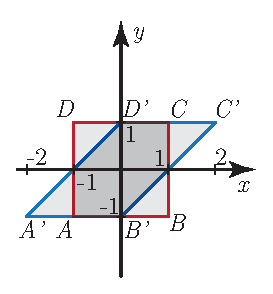
\includegraphics[scale=1]{figs/nyiras_feladat.eps}
\caption{Nyírós feladat.}
\label{fig:nyiras_feladat}
\end{figure}
\FloatBarrier


\section{Nemhomogén transzformációk}
\subsection{Homokóra nyújtós}
Mi az elmozdulásmező, a deformációs gradiens, a disztorzió és a deformáció \aref{fig:homokora_nyujtas_feladat}.\ ábrán?

\begin{figure}[htb] 
\centering    
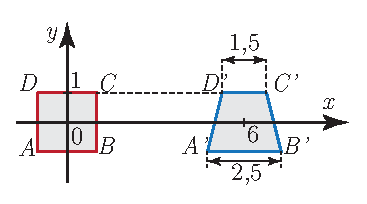
\includegraphics[scale=1]{figs/homokora_nyujtas_feladat.eps}
\caption{Homokóra nyújtós feladat.}
\label{fig:homokora_nyujtas_feladat}
\end{figure}
\FloatBarrier

\subsection{Csavarás}
Mi az elmozdulásmező, a deformációs gradiens, a disztorzió és a deformáció csavarásra? Hogyan egyszerűsödik első rendben, ha a forgatás szöge véges $z_0$ mellett infinitezimálisan kicsi?

\section{Összetett transzformációk}
\subsection{Egymásután}
\begin{enumerate}
\item Milyen transzformációk ismerhetőek fel \aref{fig:egymasutan}.\ ábráról?
\item Mi az elmozdulásmező, a deformációs gradiens, a disztorzió és a deformáció?
\end{enumerate}
\begin{figure}[htb] 
\centering    
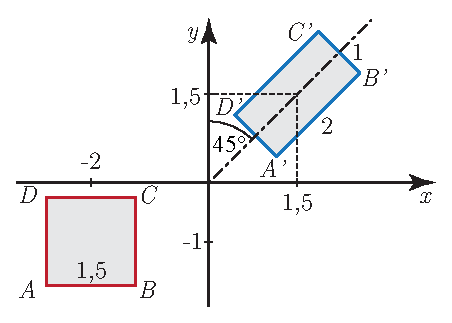
\includegraphics[scale=1]{figs/egymasutan_feladat.eps}
\caption{Egymásután.}
\label{fig:egymasutan}
\end{figure}
\FloatBarrier

\subsection{Visszafejtés}
Milyen transzformációkat takarnak az egyes deformációs gradiensek? Mekkora forgatást és milyen tengely irányú mekkora nyújtást vagy nyírást tartalmaznak? Rajzold le, mivé transzformálódik az egységnégyzetet, és jelöld be rajta a nyújtás tengelyeit és a forgatás szögét, ha van!

\[{{\mathbf{F}}_1} = \left( {\begin{array}{*{20}{c}}
  {\sqrt 2 }&-{\sqrt 2 } \\ 
  {\sqrt {0,125} }&{ \sqrt {0,125} } 
\end{array}} \right)\quad {{\mathbf{F}}_2} = \left( {\begin{array}{*{20}{c}}
  {1,2}&0 \\ 
  0&{1,5} 
\end{array}} \right)\quad {{\mathbf{F}}_3} = \left( {\begin{array}{*{20}{c}}
  2&{0,2} \\ 
  {0,2}&{0,5} 
\end{array}} \right)\]

\section{Rugalmas testek egyensúlya}
\subsection{Kocka és átlója}
\Aref{fig:kocka_atloval}.\ ábrán látható, konstans $\rho$ sűrűségű rugalmas kocka egyensúlyi állapotában a feszültségtenzor alakja 
\[{\mathbf{\sigma }}\left( {\mathbf{r}} \right) = c \left( {\begin{array}{*{20}{c}}
  {{x}}&0&0 \\ 
  0&{{y}}&0 \\ 
  0&0&{{z}} 
\end{array}} \right).\]
A kocka minden pontjában a sűrűséggel arányos, a térben nem feltétlen homogén tömegerő hat. Hat valamint minden oldallapra külön-külön állandó nagyságú és irányú felületi erősűrűség. Mekkora nagyságú és irányú
\begin{enumerate}
\item tömegerő-sűrűség hat a kockára?
\item erő hat a kocka egyes oldallapjaira?
\item erő hat az $n = \left( {1,0,1} \right)/\sqrt 2 $ normálisú, a két lapátlóra illeszkedő $ABGH$ síkra?
\end{enumerate}
\begin{figure}[htb] 
\centering    
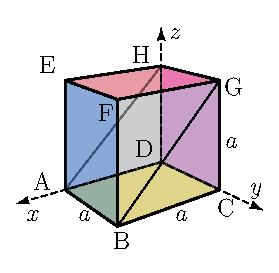
\includegraphics[scale=1]{figs/kocka_atloval.eps}
\caption{A kocka $BCGF$ és $ADHE$ lapátlóira, az $ABGH$ pontokra egy $n = \left( {1,0,1} \right)/\sqrt 2 $ normálisú síklapot fektetünk. }
\label{fig:kocka_atloval}
\end{figure}
\FloatBarrier

\subsection{Oszlopban állandó nyomás}
Egy állandó $\rho$ sűrűségű oszlop felső lapja a felfüggesztéshez van rögzítve, alsó síklapjára egy $G$ súlyú test van rögzítve, keresztmetetszete minden magasságban kör. Milyen alakú legyen, hogy a nyomás minden keresztmetszetében állandó legyen?

\section{Folyadékok I}
\subsection{Parafa-rugó}
Egy vízzel telt edénybe $d$ átmérőjű, $\rho$ sűrűségű ($\rho<\rho_{\text{víz}}$) parafagolyót helyezünk, majd az edény aljához kötjük egy $D$ rugóállandójú rugóval. Mekkora a rugó megnyúlása, ha a golyó teljes egészében a folyadékban van?

\subsection{Mérleg}
Egy érzékeny kétkarú mérleg egyik serpenyőjébe egy nagy, vízzel félig telt főzőpoharat teszünk, majd másik oldalon súlyokkal kiegyensúlyozzuk. Mit mutat a mérleg, ha a főzőpohárban lévő vízbe -- a pohárhoz való hozzáérés nélkül -- lógatunk egy testet, aminek a sűrűsége a víznél
\begin{enumerate}
\item kisebb,
\item megegyező,
\item nagyobb?
\end{enumerate}

\subsection{Hihigany}
Egy csonkakúp-alakú test a szimmetriatengelyével függőlegesen úgy úszik egy higanyt tartalmazó edényben, hogy térfogatának negyede merül a higanyba.
\begin{enumerate}
\item A magyar helyesírás szabályainak megfelele-e a "csonkakúp-alakú" kifejezés?
\item Mekkora része merülne a higanyaba a testnek, ha annyi vizet töltenénk az  edénybe, hogy az elfedje a csonka kúpot?
\end{enumerate}


\subsection{Lapát}
Egy lapát sűrűségét szeretnénk meghatározni azáltal, hogy tudjuk, hogy egyik végénél fogva, a vízbe ferdén belelógatva épp a lapát hosszának felénél van a vízszint. Ehhez azt a modellt használjuk, hogy a lapát és a víz sűrűsége állandó, alakja \sout{kecses} vékony rúd, amelynek a vastagsága elhanyagolható, továbbá a lapátot tartó kezünk gömbcsuklóként, egyetlen pontban tartja a lapátot.


\section{Folyadékok II}
\subsection{BernoUlli}
Egy szögletes, alul vízszintes, oldalt függőleges szárú, U alakú, két végén nyitott csőben folyadék van (lásd \aref{fig:ucsoves}.\ ábrát). A cső vastagsága elnyagolható a hosszáhosz képest. A csövet az U egyik szára tengelyében állandó $\omega$ szögsebességgel forgatjuk. A forgástengelyhez közelebbik vízszint helyzetét jelöli $A$, a forgástengelytől távolabbikat $B$. Hogyan viszonyul a vízszint különbsége az $A$ és $B$ pontok között az $\omega$ szögsebesség függvényében?

\begin{figure}[htb] 
\centering    
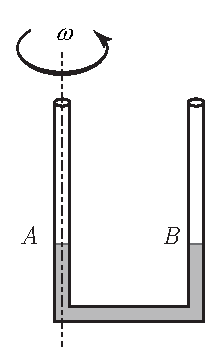
\includegraphics[scale=1]{figs/bernoUlli.eps}
\caption{Egy U alakú csőben folyadék van egyensúlyban, majd megforgatjuk a csövet az U egyik szára tengelyében.}
\label{fig:ucsoves}
\end{figure}
\FloatBarrier

\subsection{Csöves 2}
Egy U alakú, $d$ átmérű, kör keresztmetszetű nyitott csőben folyadék van, $L$ hosszban, $d \ll L$. Az egyik csövön egy pillanatra levegőt befújva egy kicsit lecsökkentjük a folyadékszint magasságát $x_0$-val, majd figyeljük a vízszint mozgását. Milyen mozgást fog végezni? Tételezzük fel, hogy a cső adott keresztmetszete mentén lévő folyadékrészre a sebességével arányos súrlódási erő lép fel.
\begin{figure}[htb] 
\centering    
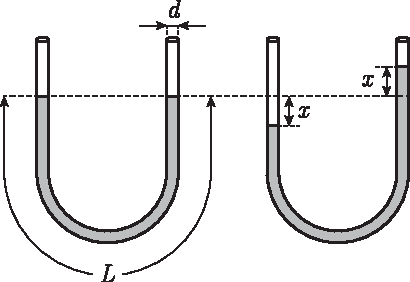
\includegraphics[scale=1]{figs/ucsoves2.pdf}
\caption{Egy U alakú csőben már megint folyadék van.}
\label{fig:ucsoves2}
\end{figure}
\FloatBarrier

\fi
\end{document}